\documentclass[12pt]{article}
\usepackage[margin=1.0in]{geometry} %page layout
\usepackage[usenames,dvipsnames]{color} %color
\definecolor{light-gray}{gray}{0.95}
\definecolor{darkgreen}{rgb}{0,0.4,0}
\usepackage{graphicx, subfigure} %figures
\usepackage{url, hyperref} %cross-referencing
\usepackage{amsmath, amssymb} %math
\usepackage{listings} %source code
\lstset{breaklines=true,
breakindent=0pt,
prebreak=\mbox{\tiny$\searrow$},
postbreak=\mbox{{\color{blue}\tiny$\rightarrow$}},
numbers=left,
commentstyle=\color{darkgreen},
numberblanklines=false,
frame=single,
captionpos=b,
backgroundcolor=\color{light-gray}}
\usepackage[3D]{movie15} %for movies (needs hyperref)
	\newenvironment{changemargin}[2]
	{
	  	\begin{list}{}
		{
			\setlength{\topsep}{0pt}%
			\setlength{\leftmargin}{#1}%
			\setlength{\rightmargin}{#2}%
			\setlength{\listparindent}{\parindent}%
			\setlength{\itemindent}{\parindent}%
			\setlength{\parsep}{\parskip}%
		}
	  	\item[]
		}
		{\end{list}
	}
\author{Salman Aslam\\Georgia Tech}
\title{VC Dimension of RVQ}
\author{Salman Aslam\\ Georgia Institute of Technology}
\date{}
\definecolor{darkgreen}{rgb}{0,0.5,0}
\newcommand{\Ntrg}{\big[N_{t=1, m=1} + \lambda \big] + \big[N_{t=1, m=2} + \lambda \big] + \ldots + \big[N_{t=1, m=M} + \lambda \big]}
\newcommand{\jointcnt}{\sum\limits_{n_{trg}=1}^{N_{trg}}I(X_t=x_t, X_{t-1}=x_{t-1})}
\newcommand{\singlecnt}{\sum\limits_{n_{trg}=1}^{N_{trg}}I(X_{t-1}=x_{t-1})}
\newcommand{\singlep}{p(X_{t-1}=x_{t-1})}
\newcommand{\singlepone}{p(X_{t-1}=1)}
\newcommand{\singleptwo}{p(X_{t-1}=2)}
\newcommand{\singlepM}{p(X_{t-1}=M)}
\newcommand{\condp}{p(X_t=x_t | X_{t-1}=x_{t-1})}
\newcommand{\jointp}{p(X_t=x_t, X_{t-1}=x_{t-1})}
\newcommand{\KmeansOuterSum}{\sum\limits_{k=1}^K}
\newcommand{\KmeansInnerSum}{\sum\limits_{{i=1 \atop x_i \in \mathcal{K}_k}}^N}
\newcommand{\KmeansSum}{\KmeansOuterSum \KmeansInnerSum}
\newcommand{\RVQInnerSum}{\sum\limits_{{i=1 \atop g_i \mapsto m_{\tau, s}}}^N}
\newcommand{\RVQOuterSum}{\sum_{s=1}^S}
\newcommand{\RVQsum}{\KmeansOuterSum \sum\limits_{{i=1 \atop g_i \in \mathcal{K}_k}}^N}
\newcommand{\KmeansInner}{{(x_i - \mu_k)}^2}
\newcommand{\RVQinner}{            {(x_i  - \hat{\mu}^{(k)})}^2}
\newcommand{\RVQinneralternate}{{(g_i - m_\tau^{(k)})}^2}
\newcommand{\RVQinneralternatealternate}{{(g_i - m_{\tau, s})}^2}
\newcommand{\KmeansError}{\KmeansSum \KmeansInner}
\newcommand{\RVQerror}     {\KmeansSum \RVQinner}
\newcommand{\RVQerroralternate}{\RVQsum \RVQinneralternate}
\newcommand{\RVQunit}{x_i -\bigg(\sum_{t=1}^Tm^{(k)}_t\bigg)}
\newcommand{\RVQequivalentCodevector}{\sum_{t=1 }^Tm^{(k)}_t}
\newcommand{\RVQequivalentCodevectorBroken}{\sum_{t=1 \atop t \neq \tau}^Tm^{(k)}_t+ m^{(k)}_\tau}
\newcommand{\RVQmultipleKmeans}{x_i -\bigg(\RVQequivalentCodevectorBroken\bigg)}
\newcommand{\RVQmultipleKmeansone}{x_i -\sum_{t=2}^Tm^{(k)}_t+ m^{(k)}_1\bigg)}
\newcommand{\RVQmultipleKmeansonealternate}{\bigg(x_i -\sum_{t=1 \atop t \neq \tau}^Tm^{(k)}_t\bigg) - m^{(k)}_\tau}
\newcommand{\RVQmultipleKmeanstwo}{x_i -\bigg(\sum_{t=1 \atop t \neq 2}^Tm^{(k)}_t+ m^{(k)}_2\bigg)}
\newcommand{\RVQmultipleKmeansT}{x_i -\bigg(\sum_{t=1}^{T-1}m^{(k)}_t+ m^{(k)}_2\bigg)}
\newcommand{\EucMatrix}
{
\left[
\begin{array}{lll}
r_{11} & r_{12} & t_x \\ 
r_{21} & r_{22} & t_y \\ 
0 & 0 & 1 \\ 
\end{array}
\right]
}	

\newcommand{\SimMatrix}
{
\left[
\begin{array}{lll}
sr_{11} & sr_{12} & t_x \\ 
sr_{21} & sr_{22} & t_y \\
0 & 0 & 1 \\ 
\end{array}
\right]
}

\newcommand{\AffMatrix}
{
\left[
\begin{array}{lll}
a &b & t_x \\ 
c & d & t_y \\
0 & 0 & 1 \\
\end{array}
\right]
}

\newcommand{\ProjMatrix}
{
\left[
\begin{array}{lll}
h_{11} & h_{12} & h_{13} \\ 
h_{21} & h_{22} & h_{23} \\ 
h_{31} & h_{32} & h_{33} \\ 
\end{array}
\right]
}

\newcommand{\RotMatrixTheta}
{
\left[
\begin{array}{rr}
\cos(\theta) & -\sin(\theta) \\ 
\sin(\theta) & \cos(\theta) \\ 
\end{array}
\right]
}

\newcommand{\RotMatrixPhi}
{
\left[
\begin{array}{rr}
\cos(\phi) & -\sin(\phi) \\ 
\sin(\phi) & \cos(\phi) \\ 
\end{array}
\right]
}

\newcommand{\RotMatrixminusPhi}
{
\left[
\begin{array}{rr}
\cos(-\phi) & -\sin(-\phi) \\ 
\sin(-\phi) & \cos(-\phi) \\ 
\end{array}
\right]
}


\newcommand{\EigenvalueMatrix}
{
\left[
\begin{array}{cc}
\lambda_1 & 0\\
0 & \lambda_2
\end{array}
\right]
}

\newcommand{\bigMatrix}
{
s \left[
\begin{array}{cc}
 (r)(a) + b &  (r)(d) - c \\
 (r)(c) - d &  (r)(b) + a
\end{array}
\right]
}


\newcommand{\bigMatrixTwo}
{
\left[
\begin{array}{cc}
(\lambda_2) p + (\lambda_1) q & (\lambda_2) s  - (\lambda_1) r \\
(\lambda_2) r  - (\lambda_1) s & (\lambda_2) q + (\lambda_1) p
\end{array}
\right]
}
\newcommand{\dr}{(\mathbf{x}_i-\boldsymbol\mu_k)^T(\mathbf{x}_i-\boldsymbol\mu_k) + \lambda({Q_{\textrm{max}}-Q_i})}

\begin{document}
\maketitle
\rule[0pt]{\textwidth}{1pt}
\tableofcontents
\rule[0pt]{\textwidth}{1pt}

%================================
\section{Introduction}
%================================
The concept of VC dimension was introduced by Vapnik~\cite{1999_BOOK_PRML_Vapnik} as a means of specifying the generalization ability of classifiers.  In this work, we look at some definitions leading up to the VC dimension.  It has been shown that the VC dimension of a nearest neighbor classifier is equal to the number of reference points in the training set~\cite{2003_JNL_PRML_Karacali}.  We extend this to show that the VC dimension of an RVQ classifier depends on both its number of stages $Q$ and the number of code-vectors per stage $M$.

%================================
\section{Theory}
%================================
In pattern recognition, a \emph{classifier} $g(x)$ is a function that maps $x_i \in \mathbb{R}^D$ to a set of $M$ discrete \emph{class} labels, $\theta  \in \{1, 2, \ldots M\}$, i.e., $g(x):~\mathbb{R}^D~\rightarrow~\{1, 2, \ldots M\}$.  The classifier errs if $g(x) \neq \theta$~\cite{1996_BOOK_PR_DevroyeGyorfiLugosi}.  Since it is not possible to create a classifier that always achieves perfect mapping, we create a probabilistic setting and let $\mathbf{X} \times \mathbf{\Theta}$ be an $\mathbb{R}^D \times \{1, 2, \ldots M\}$-valued random pair.  

\begin{enumerate}
\item \underline{Risk}.  The probability of error for estimator $g(x)$, the {\color{blue}\emph{risk}} is

\begin{equation}
\boxed{
{\color{blue}R(g)} = \mathbf{P}(g(\mathbf{X}) \neq \mathbf{\Theta})}
\label{Eqn:loss}
\end{equation}

\item \underline{Bayes Risk}. In Equation~\ref{Eqn:loss}, the minimal probability of error $\mathbf{P}^*$ is called the \emph{Bayes error} or the \emph{Bayes risk}.  

\item \underline{Bayes Classifier}.  In Equation~\ref{Eqn:loss}, the best classifier $g^*$ is called the \emph{Bayes classifier} or the \emph{Bayes rule}, and is given by

\begin{equation}
g^* = \arg\min_{\tiny g:~\mathbb{R}^D~\rightarrow~\{1, 2, \ldots M\}} {\color{blue}R(g)}
\end{equation}

\item \underline{Empirical risk}. In practical situations, $\mathbf{P}(g(\mathbf{X}) \neq \mathbf{\Theta})$ is generally unknown, and therefore so is $g^*$.  However, we assume that we have $N$ i.i.d. random pairs of training data, $\{(x_1, \theta_1), (x_2, \theta_2), \ldots, (x_N, \theta_N)\}$ with the same distribution as $p(\mathbf{X},\mathbf{\Theta})$.  The empirical risk function for this data is $R_N$, or $R(g_N)$~\footnote{The quantity $\mathbb{E}\left[R_N\right]$ is marginally useful since it is the quality of an average data sequence and not the data sequence at hand.  A \emph{consistent} classifier is one for which $\lim\limits_{N \rightarrow \infty}\mathbb{E}\left[R_N\right] = R^*$~\cite{1996_BOOK_PR_DevroyeGyorfiLugosi}.}.
  
\item \underline{Empirical risk minimization}.
Since we cannot find $g^*$, we change the setting and define $R$ as being the risk of the best classifier in class $\mathcal{C}$, for instance, all $k$-nearest neighbor classifiers with all possible values of $k$.  Then,

\begin{equation}
R \triangleq \inf\limits_{g_N \in \mathcal{C}} \mathbf{P}(g_N(\mathbf{X}) \neq \mathbf{\Theta})
\end{equation}

Using \emph{empirical risk minimization}~\cite{1999_BOOK_PRML_Vapnik}, we select a classifier $g_N$ from a class $\mathcal{C}$ by minimizing, 

\begin{equation}
\frac{1}{N} \sum\limits_{n=1}^N I_{g_N(x_n \neq \theta_n)}
\end{equation}

then the corresponding risk $R_N$ satisfies the following inequality for all $\epsilon > 0$

\begin{equation}
\mathbf{P}(R_N > R + \epsilon) \leq 8(N^V + 1) e^{-N\epsilon^2/128}
\end{equation}

where $V$ is the Vapnik Chervonenkis (VC) dimension.  The concept of VC dimension is related to \emph{shattering}.

\item \underline{Shattering}.  In the two-class classification problem, a given set of $h$ points can be labeled in $2^h$ ways.  If, for all possible labelings, a classifier $g(x)$ from the class $\mathcal{C}$ can be found which correctly assigns those labels, then we say that the set of $h$ points is shattered by the class $\mathcal{C}$~\cite{1998_JNL_SVM_Burges}.  An example of shattering in $\mathbb{R}^2$ is given in Figure~\ref{fig:shattering}.

\item \underline{VC dimension}.  If a classifier class $\mathcal{C}$, such as the class of linear classifiers, or the class of $k$-nearest neighbors with different values of $k$, has VC dimension $h$, then there exists at least one set of $h$ points that can be shattered by it, but in general, not every set of $h$ points can be shattered by the class~\cite{1998_JNL_SVM_Burges}.  For instance, in Figure~\ref{fig:shattering}, three collinear points cannot be shattered by a line.

\item \underline{Nearest neighbor classifier}.  The most popular nonparametric classifier is the nearest neighbor classifier that assigns the class label of the nearest neighbor in the training set to unknown data~\cite{2003_JNL_PRML_Karacali}.  For the nearest neighbor rule, for all distributions, the risk $R_{1NN}$ is bounded above by twice the Bayes risk,

\begin{equation}
\lim\limits_{N \rightarrow \infty} \sup\mathbb{E}\left[R_{1NN}\right] \leq 2R^*  
\end{equation}

In this sense, half of the available information in an infinite collection of classified samples is contained in the nearest neighbor~\cite{1967_JNL_PRML_Cover, 1996_BOOK_PR_DevroyeGyorfiLugosi}. 

								\begin{figure}[t]
								\centering
								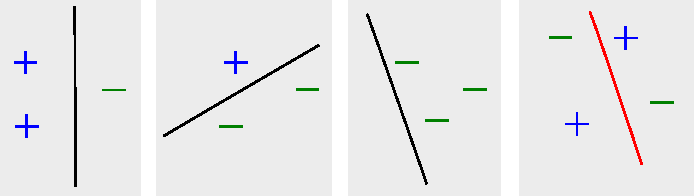
\includegraphics[width=1.0\textwidth]{figs/theory_PRML_shattering.pdf}
								\caption{A linear classifier in $\mathbb{R}^D$ can shatter $D+1$ points.  Here, in the first 3 examples, a line in $\mathbb{R}^2$ is able to shatter 3 points.  However, in the fourth example, it is unable to shatter 4 points.}
								\label{fig:shattering}
								\end{figure}

\item \underline{VC dimension of NN classifier}.   It has been shown by Kara\c{c}ali and Krim~\cite{2003_JNL_PRML_Karacali} that the VC dimension of the NN classifier is given by the number of reference points in the training set~\cite{2005_CNF_ML_Angiulli}.

\end{enumerate}

%================================
\section{VC dimension of RVQ classifier}
%================================
The reference points in the training set for a NN classifier mentioned in~\cite{2005_CNF_ML_Angiulli} c

In~\cite{2005_CNF_ML_Angiulli}, the reference points in the training set for a NN classifier corresponds to the 


In RVQ, the reference points in the training set mentioned in~\cite{2005_CNF_ML_Angiulli} correspond to the equivalent code-vectors at the end of stage $q$.  For instance, in an RVQ codebook with $Q$ stages, and $M$ code-vectors per stage, there are $M^Q$ equivalent code-vectors.  Moreover, if we wish to examine the direct-sum code-vectors at the end of say the third stage, then there are $M^3$ of them.   The number of direct-sum code-vectors, i.e. reference points in the training set mentioned in~\cite{2003_JNL_PRML_Karacali},  increases at the end of every stage.  Using the argument in, this means that the VC dimension of an RVQ nearest neighbor classifier in a variable-rate framework depends on how many stages are used.  


%================================
\section{Experiments}
%================================
In this section, we experiment with 4 RVQ decode methods:



We start with some trivial scalar examples where the training and test sets are the same.  We then move to the other extreme end of the spectrum using random data in high dimensional spaces with several observations and where the training and test sets have the same distributions but have different data.  After these experiments, we will get to tracking examples and use the likelihood formulation we have developed for RVQ.

\subsection{$S_{trg}=\{1,2,3,4,5,6,7\}$}
%-------------------------------------------------------------

\begin{table}
\centering
\subtable[3x{\color{red}\textbf 2}]{\begin{tabular}{|c|c|}\hline 
2.5  & 6\\
-1  & 1\\
-0.5  & 0.5\\\hline
\end{tabular}}\hspace{0.2in}
\subtable[2x{\color{red}\textbf 3}]{\begin{tabular}{|c|c|c|}\hline
-1 & 6 & 4\\
-1 & 1 & 0\\\hline
\end{tabular}}\hspace{0.2in}
\subtable[2x{\color{red}\textbf 4}]{\begin{tabular}{|c|c|c|c|}\hline
1 & 6.5 & 4 & 2\\
-1 & 1 & -0.5 & 0.5\\\hline
\end{tabular}}\hspace{0.2in}
\subtable[2x{\color{red}\textbf 5}]{\begin{tabular}{|c|c|c|c|c|}\hline
1 & 6.5 & 4.5 & 2 & 3\\
-0.5 & 0.5 & 0 & 0 &0\\\hline
\end{tabular}}\hspace{0.2in}
\subtable[2x{\color{red}\textbf 6}]{\begin{tabular}{|c|c|c|c|c|c|}\hline
1 & 6.5 & 4 & 2 & 3 &5\\
-0.5 & 0.5 & 0 & 0 &0 &0\\\hline
\end{tabular}}\hspace{0.2in}
\subtable[1x{\color{red}\textbf 7}]{\begin{tabular}{|c|c|c|c|c|c|c|}\hline
1 & 7 & 4 & 2 & 3 &5 &6\\\hline
\end{tabular}}
\hspace{0.2in}
\subtable[1x{\color{red}\textbf 8}]{\begin{tabular}{|c|c|c|c|c|c|c|c|}\hline
1 & 7 & 4 & 2 & 3 &5 &6&0\\\hline
\end{tabular}}
\caption{Designing RVQ codebooks with increasing code-vectors per stage, $m$ = {\color{red}\textbf {2, 3, 4, 5, 6, 7, 8}}.  The training set is $S_{trg}=\{1,2,3,4,5,6,7\}$}
\label{table:1_to_7}
\end{table}

Table~\ref{table:1_to_7} gives an example of designing RVQ codebooks for a trivial  training set in $\mathbb{R}$ that contains only 7 training points, $S_{trg}=\{1,2,3,4,5,6,7\}$.

For $m={\color{red}\textbf 2}$, case, 
For the 3x{\color{red}\textbf 2} case, 






\clearpage
\newpage
\normalsize
\bibliographystyle{ieee}
\bibliography{MyCitations}
\end{document}